\documentclass[12pt]{ctexart}
\usepackage{geometry}       % 设置页面整体布局
\geometry{top=2.5cm, bottom=2.5cm, left=2cm, right=2cm}
\usepackage{fancyhdr}       % 设置页眉页脚布局
\pagestyle{fancy}
\rhead{\thepage}            % 设置右页眉为页数
\chead{中国科学技术大学}
\cfoot{}                    % 设置中间页脚为空
\usepackage{amsmath}        % 数学公式宏包
\numberwithin{equation}{section}
\usepackage{esint}          % 交叉引用宏包
\usepackage[colorlinks,     % 设置引用的颜色
            linkcolor=black,
            anchorcolor=black,
            urlcolor=cyan,
            citecolor=black,
           ]{hyperref}
\usepackage{makecell}       % 插入表格宏包
\usepackage{longtable}      % 长表格宏包
\usepackage{appendix}       % 生成附录宏包
\usepackage{graphicx}       % 插入图片宏包
\usepackage{epstopdf}       % 插入eps图片宏包
\usepackage{cite}           % 文献引用宏包
\renewcommand{\thefigure}   % 设置图片编号格式
    {\thesection{}.\arabic{figure}}
\renewcommand{\thefootnote}{} % 设置角标编号不出现在文中
                            % 以\footnotetext{Footnotetext without footnote mark}使用
\usepackage{unicode-math}
\usepackage{listings}
\usepackage{hyperref}



\CTEXsetup[format={\Large\bfseries}]{section}

\begin{document}

\nocite{*}

\begin{center}
    \heiti \fontsize{24pt}{0}{水—正丙醇双液系气液平衡相图的绘制}

    \vspace{12pt}

    \kaishu \fontsize{13.75pt}{0}禤科材
    

    \footnotetext{\textbf{实验日期:}2022年12月16日}
    \footnotetext{\textbf{作者简介:}禤科材(2002-),男,学号PB20030874,中国科学技术大学本科在读,专业方向为化学物理}
    \footnotetext{\textbf{联系方式:}电话 18108064415 ,邮箱 \href{mailto:ustcxkc@mail.ustc.edu.cn}{ustcxkc@mail.ustc.edu.cn}}

    \vspace{5pt}

    \songti \fontsize{12pt}{0}(中国科学技术大学化学与材料科学学院,安徽 合肥 230026)
\end{center}


\noindent\textbf{摘~~~\!要}~~~\!
二组分体系相图描绘了双组分平衡体系各变量间的关系,具有重要意义。
在封闭体系中,溶液与其气相平衡后有确定的组成。本实验中使用沸点仪
测量不同组成的液相沸点,并使用安东帕折光仪间接获得了气液两相中各
组分的含量,从而绘制成水—正丙醇二组分相图。实验结果较好,与理论值
接近。
\newline
\textbf{关键字}~~~\!
沸点仪;安东帕折光仪;水—正丙醇二组分相图

\begin{center}
    {\LARGE\rmfamily\textbf{Drawing of Gas-Liquid Equilibrium Phase Diagram of Water-Propanol Two Liquid System}}

    \vspace{12pt}

    {\slshape Xuan Kecai}

    \vspace{5pt}

    (School of Chemistry and Material Science, USTC, Hefei 230026, China)
\end{center}

\noindent\textbf{Abstract}~~~\!
The phase diagram of two-component system depicts the
relationship between the variables of two-component
equilibrium system, which is of great significance. In a
closed system, the solution has a definite composition after
equilibrium with its gas phase. In this experiment, the
boiling point of liquid phase with different composition
is measured by boiling point instrument, and the content
of each component in gas-liquid two-phase is obtained
indirectly by Anton Paar refractometer, so as to draw the
two-component phase diagram of water-n-propanol. The
experimental results are good and close to the theoretical
values.
\newline
\textbf{Keywords}~~~\!
Boiling point meter; Anton Paar refractometer;
Water-n-propanol binary phase diagram

\section{序言}
在常温下,两液态物质混合而成的体系称为双液系。两液体若只能在一定
比例范围内互相溶解,称为部分互溶双液系,若两液体能以任意比例相互
溶解,则称为完全互溶双液系。

常温下,水—正丙醇体系是完全互溶双液系,其沸点不仅与外压有关,还与
双液系的组成有关。在一般情况下,双液系的气相组成和液相组成并不
相同。将双液系的沸点对其气相、液相组成作图,就可以得到双液系的
$T\sim x(y)$相图。在本实验中,使用沸点仪可以将气液两相分开从而
分别测量其组成。通过测定双液体系的折光率,依据工作曲线可以反推出其
对应的两相组成。

由于实验环境不是标准大气压,测量的沸点并非液体的正常沸点,故使用
下式对温度进行校正。
\begin{gather}
    \Delta t / ^\circ\text{C}
    = \frac{(273.15 + t/^\circ\text{C})}{10}
    \cdot \frac{(101325 - P/\text{Pa})}{101325}. \\
    t_{\text{沸}} = t_{\text{观}} + \Delta t.
\end{gather}

\section{实验}
\subsection{试剂与仪器}
蒸馏水、正丙醇(AR,国药集团化学试剂有限公司)。

YP-2B型精密稳流电源(南京南大万和科技有限公司)、DZTW型电子调温
加热套(邦西(上海)仪器科技有限公司)、Abbemat 300 Refractometer
(Anton Paar)、MKT50数字式温度计(Anton Paar)、升降底座
(天津天之丽科教仪器制造有限公司)、移液管(2mL、5mL、10mL、20mL、
50mL)、沸点仪、擦镜纸。

\subsection{实验方法}
\subsubsection{工作曲线的测定}
配制质量百分比为10\%、20\%、30\%、40\%、50\%、60\%、70\%、
80\%、90\%的正丙醇水溶液各5g,准确称量正丙醇和水的质量,测量溶液
的折光率。

\subsubsection{测定正丙醇的沸点}
安装实验体系,向沸点仪中准确移入正丙醇溶液50.00mL,使电加热丝和
温度探头均全部浸没在溶液中,打开冷却水和电源,调节电压控制为15V,
使液体沸腾,测量沸点,此时气相会冷凝到左侧的支管处。用干燥的滴管中
液相和气相冷凝液,冷却,测量折光率。

\subsubsection{测定不同双液系组成的沸点}
用移液管移取0.5mL水从支管加入烧瓶,用与2.2.2节相同的方法测量
新体系中的液相、气相的折光率和平衡时的沸点。再依次向烧瓶中加入
1mL、1.5mL、2mL、2.5mL、4mL、1.5mL的水,逐一进行测量,分别得到
不同组成时的气相、液相的折光率及各自的沸点,直到气液两相折光率
基本相等,表示已经达到最低恒沸点。

\subsubsection{反向测量}
向沸点仪中准确移入40.00mL蒸馏水,并逐一加入0.5mL、1mL、1.5mL、
2mL、4mL、10mL、20mL的正丙醇,改变体系的总组成,用与2.2.2节和
2.2.3节相同的方法测量气液平衡时各个样品的折光率和沸点,绘制相图。

\section{结果与讨论}
\subsection{实验结果}
由于实验时间恰逢疫情政策调整,本实验的操作线下完成,而理论部分线上完成。虽然实验数据老师有上传,但作者发现自己实验操作做出的数据也较好,故仍然使用当日操作所得数据。

如图 3.1 所示为水—正丙醇双液系的气液平衡相图,得到二组分的最低
恒沸点为87.406$^\circ$C,对应的正丙醇含量为63.41\%,与理论值最低
恒沸点87.7$^\circ$C接近$^{[2]}$,误差为-0.34\%,与理论正丙醇含量
69$\sim$71\%相比偏小。

\begin{figure}[!h]
    \centering
    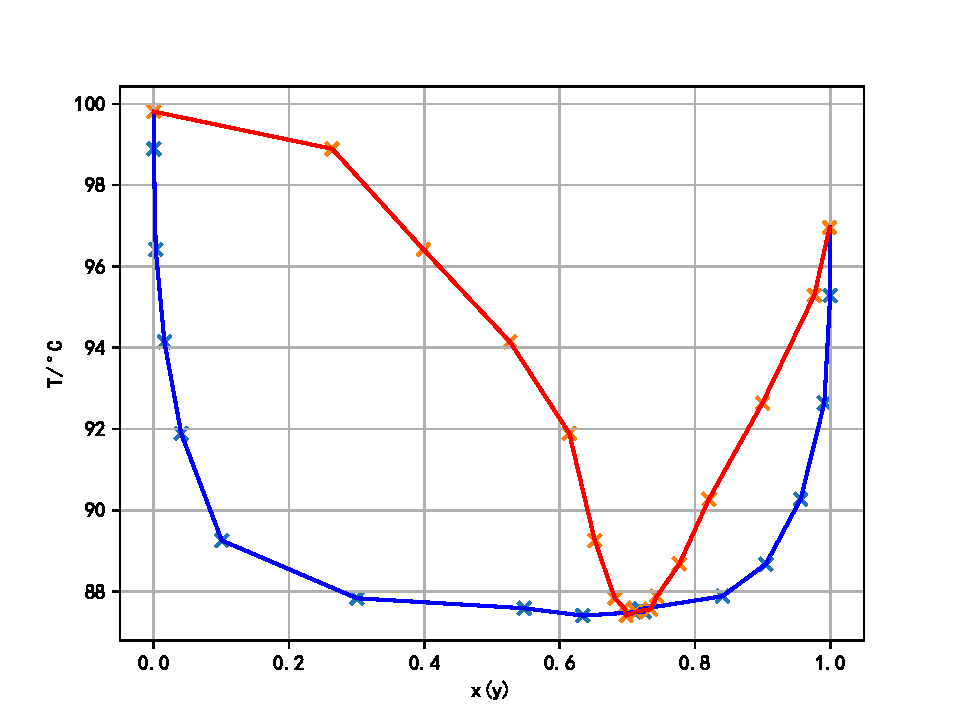
\includegraphics[scale=1.0]{xiangtu.pdf}
    \caption{水—正丙醇双液系的气液平衡相图}
\end{figure}

\subsection{误差分析}
\subsubsection{系统误差}
(1) 沸点仪、温度控制器、测温仪、折光仪等仪器本身具有一定误差。

(2) 正丙醇易挥发,挥发会使体系的正丙醇含量变小,从而使相图右半边
无法达到100\%,最低恒沸点对应组成也会在相图中左移。

(3) 实验环境的误差,实验时大气压并不精确恒定。

(4) 对工作曲线不同的拟合方法会造成误差。

\subsubsection{偶然误差}
(1) 相图由两人合作完成。不同实验人员的操作习惯会造成一定的误差。

(2) 测温仪有滞后效应,这使得测量的沸点值会有一定误差。

(3) 液体混合不均匀,导致双液体系温度不均匀,造成实验误差。

\subsection{实验改进与思考}
实验可向体系中加入小磁子,以辅助搅拌,使体系温度均一,减小误差。
可给实验装置加装恒压滴液漏斗,以减少加水/正丙醇时有机物的挥发。

\section{结语}
本实验通过测定不同组成下的双液系沸点及其气液相组成绘制出了气液平衡
相图。体系的最低恒沸点为 87.406$^\circ$C,对应的正丙醇含量为
63.41\%,与理论值最低恒沸点为 87.7$^\circ$C 接近,相对误差为
-0.34\%,与理论正丙醇含量69$\sim$71\% 相比偏小,这是由于正丙醇
挥发性强导致测量结果偏小,整体上实验精度较好,实验的可行性和操作性
较好。

\begin{center}
    \Large\bfseries{参考文献}
\end{center}
\noindent
[1] 傅献彩, 沈文霞, 姚天扬等. 物理化学(第五版). 上册[M].
高等教育出版社,2006.

\noindent
[2] J.A. 迪安, 迪安, Dean, et al. 兰氏化学手册 [M]. 科学出版社,
2003.

\newpage

\begin{center}
    \LARGE\bfseries{附录~~~实验数据处理}
\end{center}
\begin{center}
    \Large\bfseries{附录I~~~实验数据处理}
\end{center}

\subsection*{I.1~~~工作曲线的绘制}
尝试发现,用二次函数进行拟合的效果最好。拟合得到工作曲线的方程为
\begin{align}
    y = -0.0373 x^2 + 0.0870 x + 1.3334
    \tag*{(I.1)}
\end{align}
其中$x$为正丙醇质量分数,$y$为溶液折光率。作图可得如下图象。
\begin{figure}[!h]]
    \centering
    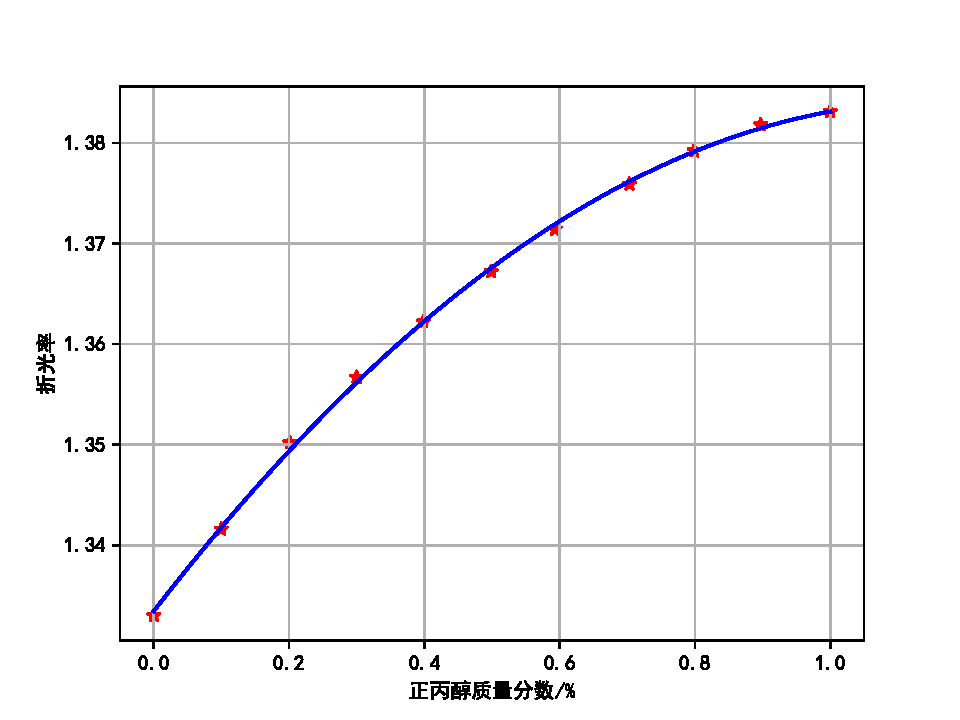
\includegraphics[scale=1.0]{gongzuoquxian.pdf}
    \caption{工作曲线}
\end{figure}

\subsection*{I.2~~~相图的绘制}
用下式对温度进行校正。
\begin{gather}
    \Delta t / ^\circ\text{C}
    = \frac{(273.15 + t/^\circ\text{C})}{10}
    \cdot \frac{(101325 - P/\text{Pa})}{101325}.
    \tag*{(I.2)} \\
    t_{\text{沸}} = t_{\text{观}} + \Delta t.
    \tag*{(I.3)}
\end{gather}
并用附录 I.1 中拟合的曲线计算体系的组成。选用数据如下表所示。

\begin{longtable}{ccccccc}
    \caption{相图绘制数据} \\
    \hline
    组别 & 平均沸点/$^\circ$C & 校正沸点/$^\circ$C & 液相折光率 & 液相组成x & 气相折光率 & 气相组成y \\
    \hline
     1 &  97.353 & 96.957 & 1.3831 & 0.9992 & 1.3831 & 0.9992 \\
     2 &  95.680 & 95.286 & 1.3832 & 1.0000 & 1.3828 & 0.9765 \\
     3 &  93.027 & 92.636 & 1.3830 & 0.9913 & 1.3815 & 0.8998 \\
     4 &  90.656 & 90.268 & 1.3825 & 0.9563 & 1.3797 & 0.8207 \\
     5 &  89.061 & 88.674 & 1.3816 & 0.9049 & 1.3785 & 0.7769 \\
     6 &  88.269 & 87.883 & 1.3802 & 0.8408 & 1.3775 & 0.7438 \\
     7 &  87.950 & 87.564 & 1.3767 & 0.7191 & 1.3772 & 0.7343 \\
     8 &  87.887 & 87.502 & 1.3769 & 0.7251 & 1.3765 & 0.7131 \\
     9 &  87.891 & 87.406 & 1.3736 & 0.6341 & 1.3760 & 0.6985 \\
    10 &  87.973 & 87.587 & 1.3699 & 0.5478 & 1.3759 & 0.6957 \\
    11 &  88.219 & 87.833 & 1.3562 & 0.3002 & 1.3754 & 0.6816 \\
    12 &  89.642 & 89.255 & 1.3426 & 0.1105 & 1.3743 & 0.6520 \\
    13 &  92.280 & 91.890 & 1.3369 & 0.0404 & 1.3728 & 0.6143 \\
    14 &  94.538 & 94.145 & 1.3348 & 0.0157 & 1.3689 & 0.5265 \\
    15 &  96.811 & 96.416 & 1.3332 & 0.0028 & 1.3622 & 0.3987 \\
    16 &  99.291 & 98.893 & 1.3327 & 0.0000 & 1.3538 & 0.2638 \\
    17 & 100.209 & 99.810 & 1.3325 & 0.0000 & 1.3327 & 0.0000 \\
    \hline
\end{longtable}

用上表中的数据作图,得到的相图如图 4.2 所示。
\begin{figure}[!h]
    \centering
    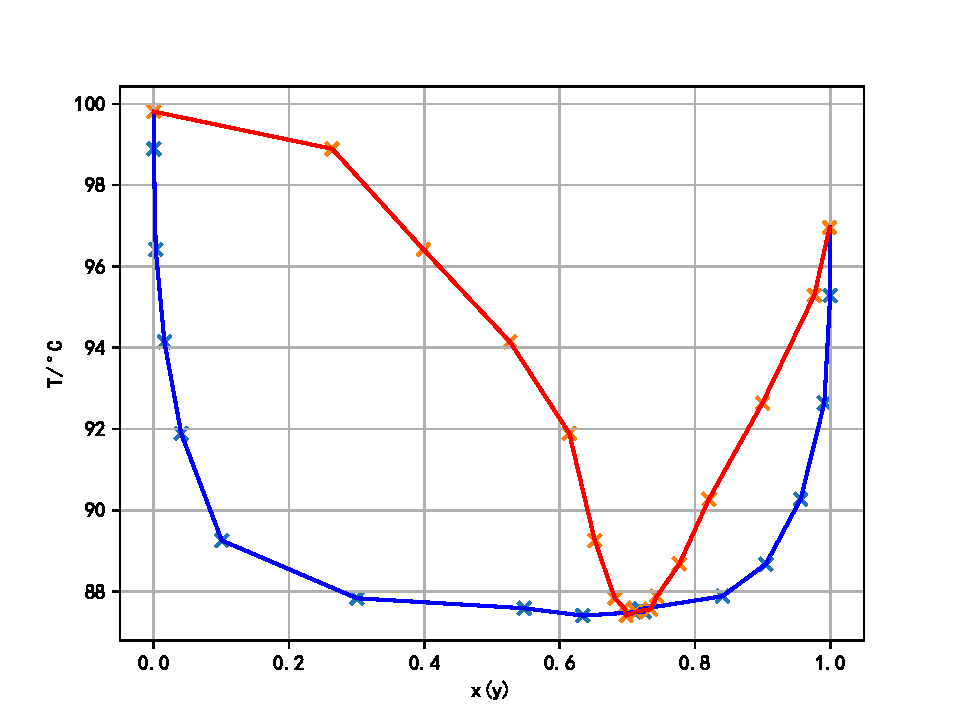
\includegraphics[scale=1.0]{xiangtu.pdf}
    \caption{水—正丙醇双液系的气液平衡相图}
\end{figure}

因此,得到二组分的最低恒沸点为 87.406$^\circ$C,对应的正丙醇含量为
63.41\%,与理论值最低恒沸点 87.7$^\circ$C 接近,相对误差为
-0.34\%,与理论正丙醇含量69$\sim$71\% 相比偏小。

\newpage
\begin{center}
    \Large\bfseries{附录II~~~原始数据记录}
\end{center}

\begin{longtable}{cccc}
    \caption{实验大气压} \\
    \hline
    组别 & 实验前 & 实验中 & 实验后 \\
    \hline
    大气压强/kPa & 102.39 & 102.41 & 102.42 \\
    \hline
\end{longtable}

\newpage
\begin{longtable}{ccccccc}
    \caption{不同组成下液体混合物沸点和折光率的测定} \\
    \hline
    组别 & 加水体积/mL & & 沸点/$^\circ$C & & 液相折光率 & 气相折光率 \\
    \hline
    1 & 0.00 & 97.352 & 97.354 & 97.353 & 1.3831 & 1.3831 \\
    2 & 0.50 & 95.681 & 95.679 & 95.680 & 1.3832 & 1.3828 \\
    3 & 1.00 & 93.026 & 93.027 & 93.029 & 1.3830 & 1.3815 \\
    4 & 1.50 & 90.663 & 90.660 & 90.645 & 1.3825 & 1.3797 \\
    5 & 2.00 & 89.059 & 89.061 & 89.063 & 1.3816 & 1.3785 \\
    6 & 2.50 & 88.265 & 88.274 & 88.269 & 1.3802 & 1.3775 \\
    7 & 4.00 & 87.955 & 87.946 & 87.949 & 1.3767 & 1.3778 \\
    8 & 1.50 & 87.883 & 87.888 & 87.889 & 1.3769 & 1.3765 \\
    \hline
\end{longtable}

\begin{longtable}{cccc}
    \caption{工作曲线数据} \\
    \hline
    组别 & 正丙醇质量/g & 总质量/g & 折光率 \\
    \hline
    1 & 0.5052 & 5.0661 & 1.3416 \\
    2 & 1.0089 & 5.0188 & 1.3502 \\
    3 & 1.5033 & 5.0134 & 1.3567 \\
    4 & 1.9936 & 5.0041 & 1.3622 \\
    5 & 2.5033 & 5.0178 & 1.3672 \\
    6 & 3.0105 & 5.0732 & 1.3714 \\
    7 & 3.5241 & 5.0117 & 1.3759 \\
    8 & 3.9985 & 5.0047 & 1.3792 \\
    9 & 4.5108 & 5.0279 & 1.3818 \\
    \hline
\end{longtable}

\end{document}
